\documentclass[11pt,a4paper]{article}
\usepackage[T1]{fontenc}
\usepackage{lmodern,microtype}
\usepackage[margin=27mm,headheight=15pt]{geometry}
\usepackage{amsmath,amssymb,amsthm,mathtools}
\usepackage{booktabs,longtable,array,enumitem}
\usepackage{xcolor,tikz}
\usetikzlibrary{arrows.meta,calc}
\usepackage{listings}
\usepackage[hidelinks,breaklinks]{hyperref}
\usepackage{fancyhdr}
\definecolor{ink}{HTML}{18354A}
\definecolor{lightink}{HTML}{F0F4F7}
\pagestyle{fancy}\fancyhf{}
\fancyhead[L]{\small ProveIt / Unknot Recognition}
\fancyhead[R]{\small Certified cyclic braid compression}
\fancyfoot[C]{\thepage}
\setlength{\parskip}{4pt}
\setlength{\parindent}{14pt}
\setlist{nosep,leftmargin=*,topsep=5pt}
\newtheorem{theorem}{Theorem}[section]
\newtheorem{lemma}[theorem]{Lemma}
\newtheorem{proposition}[theorem]{Proposition}
\newtheorem{corollary}[theorem]{Corollary}
\theoremstyle{definition}\newtheorem{definition}[theorem]{Definition}
\newtheorem{example}[theorem]{Example}
\theoremstyle{remark}\newtheorem{remark}[theorem]{Remark}
\newcommand{\B}{\mathrm B}
\newcommand{\NF}{\operatorname{NF}}
\newcommand{\len}{\operatorname{len}}
\newcommand{\eps}{\varepsilon}
\newcommand{\rot}{\operatorname{rot}}
\newcommand{\Z}{\mathbb Z}
\newcommand{\Q}{\mathbb Q}
\newcommand{\id}{\mathrm{id}}
\newcommand{\kc}[1]{\kappa^{\mathrm{cyc}}_{#1}}
\newcommand{\kl}[1]{\kappa^{\mathrm{lin}}_{#1}}
\newcommand{\code}[1]{\texttt{\detokenize{#1}}}
\lstset{basicstyle=\ttfamily\footnotesize,breaklines=true,columns=fullflexible,
 frame=single,rulecolor=\color{ink!25},backgroundcolor=\color{lightink},
 keepspaces=true,showstringspaces=false}
\hypersetup{pdftitle={Support-Unrestricted Cyclic Braid Kernels},
 pdfauthor={ProveIt research contribution, AI-assisted draft},
 pdfsubject={Exact braid compression, explicit kernel separations, and conditional quasi-polynomial unknot recognition}}
\begin{document}
\begin{titlepage}
\vspace*{10mm}
{\color{ink}\Large PROVEIT RESEARCH NOTE\par}
\vspace{12mm}
{\color{ink}\huge\bfseries Support-Unrestricted\\[3pt] Cyclic Braid Kernels\par}
\vspace{7mm}
{\Large Shared Garside prefixes, verifiable compression,\\
strict target-radius separations, and\\quasi-polynomial recognition classes\par}
\vspace{11mm}
{\large Prepared for Vladimir Reshetnikov's ProveIt program\par}
{AI-assisted mathematical research draft\par}
{7 October 2026\par}
\vspace{9mm}
\begin{abstract}
We develop an exact, certificate-producing preprocessing layer for the
ProveIt unknot recognizer. It removes the two-generator support restriction
of the existing local braid compressor and shares one table of Garside
prefix states over every cyclic cut. A second trie shares arithmetic among
finite target words. For a fixed target radius, the resulting optimizer is
polynomial-time and returns an optimal set of disjoint substitutions for its
explicit one-pass rule set. We give bit-complexity and certificate-size bounds,
including a sharper bound in terms of the maximum canonical prefix height.

An explicit infinite family of four-strand unknots separates target radii
one and two: the radius-one cyclic kernel leaves all $4m+1$ letters,
whereas radius two leaves exactly three. The proof uses an induced lattice
path and a signed-crossing obstruction to single-letter replacements across
the remaining generator. A different family consists of geodesic
three-braid representatives of the unknot, proving that unrestricted braid
equality shortening alone cannot replace closure-aware operations.

An uncapped composition with exact Khovanov homology has quasi-polynomial
complexity on constructively recognizable small-kernel families, including
conjugated flat multi-letter inflations. We do not prove a small-kernel
bound for arbitrary unknots. The accompanying standard-library Python
implementation includes an independent local-move verifier, a cheaper
whole-word normal-form shortcut, 47 passing tests, exhaustive independent
checks, raw paired measurements, and integration instructions. Measured
speedups concern shared versus duplicated prefix algebra, not the complete
upstream recognizer.
\end{abstract}
\vfill
\noindent\colorbox{lightink}{\parbox{\dimexpr\textwidth-2\fboxsep\relax}{
\textbf{Status.} Mathematical proofs are supplied below. Implementation
validation is by independent replay and finite tests, not a Lean
formalization. No general quasi-polynomial unknot-recognition theorem or
end-to-end upstream speedup is claimed.}}
\end{titlepage}
\setcounter{tocdepth}{1}
\tableofcontents
\newpage

\section{Research context and precise scope}

\subsection{The current repository bottleneck}
The inspected ProveIt tree already contains exact Khovanov-based recognition,
structural certificates, homological windows, twist compression, component
sharing, and optional rank-two braid preprocessing
\cite{ProveItReadme,ProveItRankTwo}. Its rank-two stage is substantially more
than a heuristic cancellation pass: it optimizes disjoint replacements of
subwords supported on at most two Artin generator indices, checks exact local
braid equality, and independently replays a certificate. Its near-linear
bound exploits faithful low-rank states and bounded overlap of local
corridors. The present note does not rediscover or replace that result.

The same maintained analysis exhibits four-strand unknot words on which no
strictly shortening rank-two substitution can start. Increasing the number
of identical passes does not solve that obstruction. This suggests two
separate changes: remove the support restriction, and permit a recorded
cyclic cut before searching. The first uses classical Garside normal forms;
the second preserves a closed braid rather than the original braid element.
Keeping those two equality scopes distinct is essential.

The broader quasi-polynomial goal is not settled by such preprocessing.
Lackenby's July 2026 preprint develops hierarchical constructions but its
Section 9 explicitly does not provide enough algorithmic precision for a
running-time estimate, and leaves the required hierarchy-parameter bounds
unproved there \cite{Lackenby2026}. We neither use an unspecified hierarchy
operation as an oracle nor infer a general complexity theorem from an
announcement. Our route below is an independent, parameterized improvement
to the executable braid/Khovanov pipeline.

\subsection{What is classical, extended, and proved here}
Classical inputs are the Artin presentation of braid groups, the simple-braid
permutation model, uniqueness of the left-greedy Garside normal form, and
Khovanov detection of the unknot \cite{Dehornoy2007,KM2011}. The
prefix-table dynamic program is an extension of the repository's existing
rank-two recurrence, not an independently new general dynamic-programming
principle.

The contributions developed and proved in this note are the shared
\emph{doubled-prefix and inverse-target-trie} construction, its explicit
height-sensitive cost accounting and replay format, the unrestricted cyclic
kernel analysis, the infinite radius-one/radius-two separation, and the
constructive recognition classes obtained by composing these results.
We also give a geodesic unknot obstruction and a practical candidate portfolio.
These are new contributions to this package relative to the inspected
maintained sources. A comprehensive priority search over all braid-algorithm
literature has not been performed; global historical novelty is not asserted.

The suggested \code{openai/math} repository was inspected, including its
formalized positive-braid restriction lemma
\cite{OpenAIRestriction}. Its separation of a derivation from a support
restriction is methodologically relevant. No new theorem from that repository
is needed as an unverified premise here, and no claim is made that our Python
implementation has been checked by its Lean library.

\subsection{Claim ledger}
\begin{center}\small
\begin{tabular}{p{0.27\textwidth}p{0.64\textwidth}}
\toprule
Claim & Status and scope\\
\midrule
Exact kernel optimization & Proved for disjoint one-pass substitutions from a fixed finite dictionary, with optional cyclic rotation.\\
Polynomial preprocessing & Proved for each fixed radius, with explicit dependence on strand count and prefix height.\\
Strict radius separation & Proved on an infinite family of actual four-strand unknots.\\
Quasi-polynomial recognition & Proved for the stated small-kernel families, using an uncapped exact fallback.\\
Implementation soundness & Independently replayable local certificates; 47 passing tests. No formal verification of Python semantics.\\
Performance & Measured compressor-level costs with raw data. No complete upstream benchmark was run.\\
General quasi-polynomial bound & Not established; no universal structural hypothesis is silently assumed.\\
\bottomrule
\end{tabular}
\end{center}

\section{Braid words, kernels, and equality scopes}

Let
\[
 \B_b=\langle \sigma_1,\ldots,\sigma_{b-1}\mid
 \sigma_i\sigma_{i+1}\sigma_i=\sigma_{i+1}\sigma_i\sigma_{i+1},\quad
 \sigma_i\sigma_j=\sigma_j\sigma_i\ (|i-j|\ge2)\rangle.
\]
A word $w=a_1\cdots a_n$ is encoded by signed integers. Its literal length is
$n$, not its minimum Artin length. An empty word on one strand closes to the
unknot; an empty word on several strands is not a knot. The compressor itself
is defined for braids whether or not their closures are connected.

For a finite dictionary $D$ of literal target words, a permitted plan consists
of disjoint intervals $[i,j)$ in the original word and replacements
\[
 w[i:j]=v\quad\text{in }\B_b,\qquad v\in D,\quad |v|<j-i.
\]
Unreplaced letters are retained. The intervals are not interpreted in a word
that has already been edited. This makes a one-pass plan unambiguous and
prevents a hidden saturation loop from entering the complexity claim.

\begin{definition}[Linear and cyclic kernels]
Let $\kappa_D^{\rm lin}(w)$ be the minimum output length over such plans.
For $n>0$, put
\[
 \rot_s(w)=w[s:n]w[0:s],\qquad
 \kappa_D^{\rm cyc}(w)=\min_{0\le s<n}\kappa_D^{\rm lin}(\rot_s(w)).
\]
For the empty word the only cut is zero. The radius-$\rho$ dictionary is
\[
 D_\rho=\{v: |v|\le\rho\},\qquad
 M_\rho=|D_\rho|=\sum_{d=0}^{\rho}(2b-2)^d.
\]
We abbreviate its two optimum lengths by $\kl{\rho}$ and $\kc{\rho}$.
Literal targets representing the same braid may both remain in the dictionary;
the dynamic program accounts for their actual lengths.
\end{definition}

A cyclic cut is conjugacy, not equality: if $w=uv$, then
$vu=u^{-1}wu$. After the cut, every replacement is braid equality in its
unchanged surrounding context. Therefore a cyclic certificate proves that
the output closure is isotopic to the original closure. It does not assert
$w=\rot_s(w)$ in $\B_b$.

The optimum here is not a minimum over all braid presentations, all sequences
of length-preserving relations, or all Markov moves. It can remain large even
when the original braid has a much shorter equal word. Section~\ref{sec:rectangle}
gives an explicit infinite example. The separate portfolio stage can exploit
such an equality without mislabeling it as a radius-one plan.

\begin{lemma}[A safe stopping bound]\label{lem:lower}
Let $e(w)$ be the signed exponent sum, and let $c(\pi(w))$ be the number of
cycles of the induced permutation on $b$ strands. Every word equal to a cyclic
rotation of $w$ has length at least
\[
 L(w)=\max\bigl\{|e(w)|,\ b-c(\pi(w))\bigr\}.
\]
Consequently a search attaining $L(w)$ may stop without checking the remaining
cuts. If $L(w)=n$, the unchanged word is already optimal for every dictionary.
\end{lemma}
\begin{proof}
Each signed Artin letter contributes $\pm1$ to exponent sum. Its permutation
is one transposition, which changes the number of cycles by exactly one.
Starting from the identity permutation requires at least $b-c(\pi(w))$
transpositions. Exponent sum and permutation cycle type are conjugacy
invariants. These bounds apply to every permitted output.
\end{proof}

For a knot closure, $c(\pi(w))=1$, hence $b\le n+1$. After compression to $k$
letters without changing strand count, the same argument gives $b\le k+1$.
This removes a potentially hidden strand parameter from the recognition
corollary. Polynomial dependence on a numerically huge strand count is not
claimed to be polynomial in a succinct binary encoding of arbitrary
many-component empty braids.

\section{An exact classical Garside engine}

\subsection{Simple braids and the local transfer}
Write $\Delta=\Delta_b$ for the positive half-twist, and
$B=\binom b2$ for its Artin length. A simple positive braid crosses each pair
of strands at most once and is uniquely determined by its permutation.
We use the convention that $p[i]$ is the bottom position of top strand $i$,
with indices $0,\ldots,b-1$. This is the inverse of conventions that record
the top label seen at a bottom position.

In this convention the starting atoms of a simple braid $p$ are its descents,
and the finishing atoms are the descents of $p^{-1}$. The classical
left-greedy normal form is
\begin{equation}\label{eq:nf}
 g=\Delta^z s_1\cdots s_r,
\end{equation}
where $z\in\Z$, each $s_i$ is a nonidentity simple braid different from
$\Delta$, and every starting atom of $s_{i+1}$ is a finishing atom of $s_i$.
The existence and uniqueness of this form are classical
\cite{Dehornoy2007}. We represent it by the integer $z$ and the complete
permutation arrays, not by a quotient or a probabilistic fingerprint.

\begin{lemma}[Checkable transfer]\label{lem:transfer}
For adjacent simple factors $A,C$, an atom indexed by $i+1$ can be moved from
$C$ to $A$ whenever
\[
 C[i]>C[i+1],\qquad A^{-1}[i]<A^{-1}[i+1].
\]
The new left factor swaps the \emph{values} $i,i+1$ in $A$, and the new right
factor swaps \emph{positions} $i,i+1$ in $C$. Both remain simple and their
product is unchanged. The right factor is removed if it becomes the identity.
\end{lemma}
\begin{proof}
The first inequality says that $C=\sigma_{i+1}C'$ with
$\ell(C')=\ell(C)-1$. The second says that $A\sigma_{i+1}$ is simple,
with length $\ell(A)+1$. Uniqueness of the simple braid for a permutation
identifies the two updated arrays with these two factors. Thus
$AC=(A\sigma_{i+1})C'$. The array operations are exactly right composition
and left removal in the stated convention.
\end{proof}

A positive input letter is appended as a simple factor. For a negative letter,
use
\[
 \sigma_i^{-1}=\Delta^{-1}c_i,\qquad c_i=\Delta\sigma_i^{-1},
 \qquad S\Delta^{-1}=\Delta^{-1}\tau(S),
\]
where $\tau$ reverses the generator indices. On a permutation array,
\[
 \tau(p)[i]=b-1-p[b-1-i].
\]
We decrease $z$ by one, apply $\tau$ to all existing factors, and append $c_i$
if it is nonidentity. Transfers are then performed until every adjacent pair
is left weighted. Any half-twist factors are necessarily initial: a normal
pair with a right factor $\Delta$ requires every atom to finish the left
factor, so that factor must itself be $\Delta$. Extracting the initial
half-twists completes \eqref{eq:nf}.

\subsection{An elementary transfer potential}
\begin{theorem}[Amortized normalization cost]\label{thm:normalcost}
Normalizing a signed $m$-letter word by the described atom-transfer algorithm
uses at most
\[
 B\,m(m-1)/2
\]
transfers, at most $m$ simultaneous simple factors, and
$O(m^2b^3)$ word operations. Right-multiplying one already normal state of
$r$ factors by an atom costs $O((r+1)^2b^3)$ word operations. Integers have
$O(\log(m+b+2))$ bits during whole-word normalization.
\end{theorem}
\begin{proof}
For a temporary list of factors, indexed from zero, define
\[
 \Phi(s_0,\ldots,s_{r-1})=\sum_{j=0}^{r-1}j\,\ell(s_j).
\]
A transfer reduces $\Phi$ by exactly one before any deletion. Removing an
identity or extracting an initial half-twist cannot increase it. The
involution $\tau$ preserves simple length. Appending the $k$th input letter
increases $\Phi$ by at most $B(k-1)$, and creates at most one factor. Starting
from zero potential proves the transfer bound by summing these increases.

A transfer or a test for a transferable atom scans at most $b$ positions.
The scan index advances on a failed test and moves back by at most one after
a transfer, so the number of tests is bounded by the number of scanned
factors plus a constant multiple of the transfers. Over the entire word,
there are at most $m$ factor deletions and $m$ half-twist extractions;
even literal Python-list shifting contributes only $O(m^2)$ operations.
Copies and applications of $\tau$ cost $O(m^2b)$ in total. Since $B=O(b^2)$,
the stated $O(m^2b^3)$ bound follows.

For a single append, the initial and appended list has at most $r+1$ factors,
so its potential is $O(B(r+1)^2)$. List shifts contribute $O((r+1)^2)$,
and the same test accounting gives the second bound. The half-twist exponent
and factor indices grow at most linearly with input length; strand positions
are at most $b-1$.
\end{proof}

This bound is intentionally conservative. It establishes a polynomial exact
engine for the new optimizer; it is not a claim that this implementation
matches the best known Garside algorithms.

\subsection{Canonical height and interval states}
Let $\ell_c(g)$ denote the number $r$ in \eqref{eq:nf}, ignoring the half-twist
power. For the doubled word $ww$, let $P_j$ be its prefix product, and set
\begin{equation}\label{eq:height}
 R=\max_{0\le j\le2n}\ell_c(P_j).
\end{equation}
Always $R\le2n$; it can be much smaller.

\begin{lemma}[Height calculus]\label{lem:height}
For all braids $g,h$,
\[
 \ell_c(g^{-1})=\ell_c(g),\qquad
 \ell_c(gh)\le\ell_c(g)+\ell_c(h).
\]
Thus every interval prefix $P_i^{-1}P_j$ of $ww$ has canonical height at most
$2R$, and every target query $P_jv^{-1}$ with $|v|\le\rho$ has height at most
$R+\rho$.
\end{lemma}
\begin{proof}
To multiply two normal forms, commute the second half-twist power to the
left, applying the appropriate power of $\tau$ to the first factor list,
and concatenate the lists. Normalization does not increase the number of
factors. To invert a simple factor, write its inverse as a half-twist inverse
times a simple complement. Applying this to a list gives an inverse
representation with at most the original number of simple factors.
Applying the same inequality to $g^{-1}$ yields equality. The remaining
claims follow by subadditivity and $\ell_c(v^{-1})\le |v|$.
\end{proof}

\section{Shared prefixes and an exact cyclic optimizer}

\subsection{The endpoint identity}
For any original or doubled-word interval,
\begin{equation}\label{eq:endpoint}
 w[i:j]=v\quad\Longleftrightarrow\quad P_i=P_jv^{-1}.
\end{equation}
This is an equality of braid elements, not a conjugacy test. It holds for
all supports. In particular, it must not be replaced by equality of
permutations: pure braids would then produce false cancellations.

Compute the complete canonical states of $P_0,\ldots,P_{2n}$. Sort these
states lexicographically, remove exact duplicates, and assign integer
identifiers. Look up every state $P_jv^{-1}$ by binary search in that same
sorted table. If the state is absent, that target cannot match any start
endpoint in the doubled word. This interning is deterministic and requires
no expected-time hash-table hypothesis.

For a cut $s$, relative interval positions $i,j$ refer to global positions
$s+i,s+j$. Their products are still $P_{s+i}^{-1}P_{s+j}$. Consequently the
same global query table works for \emph{every} cut. Recomputing a normal form
of every rotated word is unnecessary; no equation requires conjugating a
query state or cyclically reducing its normal form.

\subsection{The scalar dynamic program}
Fix a cut, and write $F[j]$ for the maximum number of letters removed from
the first $j$ letters of that rotation. Immediately before processing $j$,
maintain for each canonical-state identifier $q$
\begin{equation}\label{eq:htable}
 H(q)=\max_{0\le i<j\, :\, P_{s+i}=q}(F[i]-i),
\end{equation}
with one attaining $i$. Missing entries have value $-\infty$. Then
\begin{equation}\label{eq:dp}
 F[j]=\max\left\{F[j-1],\quad
 \max_{v\in D}\bigl(j-|v|+H(P_{s+j}v^{-1})\bigr)\right\}.
\end{equation}
After all queries at $j$, insert $F[j]-j$ under the identifier of $P_{s+j}$.
The query-before-insertion order excludes empty source intervals.

\begin{theorem}[Exact one-pass optimization]\label{thm:optimal}
The recurrence \eqref{eq:dp}, with backpointers to attaining starts and
targets, returns $\kappa_D^{\rm lin}(\rot_s(w))=n-F[n]$. Taking the best
of all cuts returns $\kappa_D^{\rm cyc}(w)$. Only strictly shorter
replacements need to be recorded.
\end{theorem}
\begin{proof}
An optimal plan on a prefix either retains its last letter, contributing at
most $F[j-1]$, or ends in a replacement $[i,j)\mapsto v$. In the latter case,
all earlier replacements lie in the first $i$ letters, so its savings are
at most $F[i]+j-i-|v|$. Equation~\eqref{eq:endpoint} and the maximum in
\eqref{eq:htable} enumerate precisely these possibilities. Conversely, each
term of the recurrence extends a valid optimal prefix plan, so induction
proves equality.

If $j-i\le|v|$, its candidate savings are at most $F[i]$, and hence at most
$F[j-1]$. Such a candidate cannot strictly improve the retained-letter
choice. Choosing backpointers only on a strict improvement therefore records
only strictly shortening source intervals. Backtracking jumps from $j$ to
its chosen start $i$, so the recorded intervals are disjoint.

The outer minimum is the definition of the cyclic optimum. Equivalently,
any disjoint plan drawn on a circle can be cut at a boundary of one of its
blocks (or at any unused boundary), and is represented by one of the $n$
linear problems. A block covering the entire word also has a boundary.
\end{proof}

For radius one this extends the repository's prefix recurrence from its
faithful rank-two local states to exact global states. The innovation is
not the last-interval induction itself, but the unrestricted, shared
realization of its group queries and the associated verifiable cost model.

\subsection{Sharing the target arithmetic as well}
For a general finite dictionary, build a trie of the literal words $v^{-1}$.
Starting with $P_j$ at the root, append one signed letter along each trie
edge. The state at the terminal for $v^{-1}$ is $P_jv^{-1}$. Each trie edge
is traversed once at that endpoint. The same partial product is not
recomputed separately for all targets extending it.

The implementation constructs a deterministic depth-first trie by sorting
inverse target words and computing longest common prefixes. Only states
along the current trie branch need remain live. For the full radius-$\rho$
word ball, every prefix is itself in the dictionary, so the number of trie
nodes is exactly $M_\rho$.

\begin{theorem}[Shared algebra count]\label{thm:sharedcount}
For a nonempty word and a target trie with $T$ nodes, including the root,
the all-cut preprocessing uses exactly $2nT$ calls to the signed-atom
append operation: $2n$ for doubled prefixes and $2n(T-1)$ for target edges.
This excludes generation of the final winning certificate.

A reference implementation that freshly prepares $n$ prefixes and the same
trie for each of the $n$ rotations uses $n^2T$ such calls. Both still perform
$O(n^2|D|)$ scalar dynamic-programming work in the worst case.
\end{theorem}
\begin{proof}
The doubled word has $2n$ nonempty prefixes. At each endpoint its root state
is already available, and every nonroot trie node requires exactly one
append from its parent. These computations do not depend on the cut. The
reference repeats the analogous $n+n(T-1)=nT$ construction for each cut.
\end{proof}

The ratio of the two append counts is exactly $n/2$, not a general elapsed
speedup theorem. States for doubled prefixes can be taller than states for
individual rotations, scalar work is unchanged, and the doubled setup can
lose on the smallest inputs. Safe lower-bound stopping can reduce the
number of evaluated cuts, but the current implementation prepares the
entire query table first.

\section{Bit complexity, storage, and certificate size}

\begin{theorem}[Height-sensitive kernel bound]\label{thm:cost}
Let $n\ge1$, $b\ge2$, $\rho\ge1$, $M=M_\rho$, and let $R$ be
\eqref{eq:height}. The full radius-$\rho$ cyclic optimizer, including a
winning certificate and its independent replay, has the following
conservative word-operation bound:
\begin{align}
 T(n,b,\rho,R)=O\bigl(&nM(R+\rho+1)^2b^3
       +nM(R+\rho+1)b\log(n+2)\nonumber\\
       &+n^2M+M\rho\log(M+2)
       +n(R+\rho+1)b^3\bigr).\label{eq:cost}
\end{align}
Its search workspace, excluding the emitted proof, is
\begin{equation}\label{eq:space}
 O\bigl(n(R+1)b+nM+M\rho+\rho(R+\rho+1)b\bigr)
\end{equation}
words. A winning residual-word certificate has
$O(n(R+\rho+1)b^2)$ elementary records, and replay costs
$O(n(R+\rho+1)b^3)$ word operations.

All computations admit a bit-cost bound obtained by multiplying
\eqref{eq:cost} by
$O(\log(n+b+\rho+M+2))$. For each fixed $\rho$, the worst-case preprocessing
is polynomial in $n,b$. In particular, the leading conservative word bounds
are $O(n^3b^4)$ for radius one and $O(n^3b^5)$ for radius two, with the
logarithmic lookup and bit factors understood as in \eqref{eq:cost}.
\end{theorem}
\begin{proof}
There are $O(nM)$ signed-atom append calls. By
Lemma~\ref{lem:height}, the temporary query states have at most
$R+\rho+1$ factors. The single-append bound of
Theorem~\ref{thm:normalcost} gives the first term of \eqref{eq:cost}.

Comparing two canonical states scans at most $O((R+\rho+1)b)$ integer
entries. Sorting the original prefix table and binary-searching the target
states gives the second term, which also dominates the original-prefix
sort. Arrays for \eqref{eq:htable} and the backpointers require $O(n)$
initialization per cut and $O(nM)$ target checks per cut, giving $O(n^2M)$.
Generating and sorting the target dictionary and its trie accounts for
$O(M\rho\log(M+2))$.

For a recorded interval $u$ with target $v$, version-two certificates
normalize $uv^{-1}$ to the identity. The source intervals are disjoint, so
$\sum |u|\le n$. Strict shortening implies $\sum |v|<\sum |u|$ when
there are replacements. Thus the total number of residual letters is at
most $2n$. During the $u$ portion, every relative prefix has height at most
$2R$. During the target inverse portion it has height at most $2R+\rho$.
The potential proof now bounds the total transfers by the sum of the
per-append increases, $O(n(R+\rho+1)b^2)$, rather than by the square of the
largest interval length. Resetting to the identity between intervals
introduces no positive initial potential. Testing and replaying each
transfer costs $O(b)$; copies and list deletion shifts are covered by the
same bound. This proves the certificate and replay assertions and the last
term in \eqref{eq:cost}.

The original canonical states use $O(n(R+1)b)$ words. The query table has
$O(nM)$ integer entries, the dictionary and trie use $O(M\rho)$ words, and
only a depth-$\rho$ stack of query states need be retained during a trie
walk. The dynamic-programming arrays are smaller than these terms. This
proves \eqref{eq:space}. The proof itself is an additional output allocation,
not included in that search-workspace claim.

Permutation positions, powers, source indices, target identifiers, and
counters fit in words of the displayed logarithmic bit length. Binary
comparison, addition, and array-address bookkeeping can be implemented
within that bit factor. With $R\le2n$ and fixed $\rho$, $M=O_\rho(b^\rho)$,
which gives polynomial worst-case cost and the two stated leading terms.
\end{proof}

\begin{remark}[Parameter accounting]
The polynomial claim does not cover an arbitrary radius supplied in binary.
The target dictionary is exponential in $\rho\log(b+1)$. For a varying
radius, \eqref{eq:cost} is the operative bound. In particular, a radius that
makes $M$ quasi-polynomial can still yield quasi-polynomial preprocessing,
but not polynomial preprocessing by assertion. The finite-radius API has
an explicit target-count cap; the theorem concerns the uncapped route.
\end{remark}

\subsection{Why a cheap whole-word candidate comes first}
The optimizer solves a restricted combinatorial objective. A classical
normal form may directly expose a short equal word outside that objective.
For a normal state \eqref{eq:nf}, expand the half-twist power and each simple
factor to a reduced positive word. Its length is
\[
 |z|\binom b2+\sum_i\ell(s_i).
\]
The code computes this length before allocating the expansion and keeps it
only when it is shorter than the input. Equality is checked by a residual
certificate, just as for a dictionary replacement.

\begin{proposition}[Certified candidate portfolio]\label{prop:portfolio}
Compute this whole-word candidate first. If it attains $L(w)$, return it.
Otherwise compute the radius-$\rho$ cyclic kernel on the \emph{original}
input and return the shorter verified candidate. The portfolio output
length $k$ satisfies
\[
 k\le\kc{\rho}(w),
\]
and its closure is isotopic to the original closure. It adds only polynomial
normalization and replay overhead. It need not itself be an optimal
radius-$\rho$ plan.
\end{proposition}
\begin{proof}
If the first candidate attains the universal lower bound, its length is
no larger than the kernel optimum. Otherwise the kernel is explicitly one
of the compared candidates. The whole-word candidate is equal to the
original braid, while the cyclic candidate is equal after its recorded
rotation. Both certificates are rooted at the original word, so no
unrecorded composition of transformations is needed.
\end{proof}

This shortcut is classical algebra used responsibly, not a new Garside
theorem. It is particularly important in interpreting the radius separation
below: that family is difficult for a specific replacement dictionary,
not for every braid simplifier.

\section{Independent replay and the trust boundary}

\subsection{What is recorded}
A certificate records the strand count, a source digest, the linear or cyclic
scope, the rotation, the output, and disjoint original-coordinate source
intervals. Each interval carries its target and a per-input-letter sequence
of simple-factor transfer locations and extracted half-twist counts.
Version one specializes targets to the empty word or one signed letter;
version two checks the residual word $uv^{-1}$ against the identity.

The verifier does not import the optimizer or the normalizer. It reconstructs
its own permutation arrays, tests the two inequalities in
Lemma~\ref{lem:transfer} before every transfer, and checks every half-twist
extraction literally. Negative input letters use the explicit complement
and $\tau$ formulas, not an asserted intermediate normal state. A successful
version-two replay must end with exponent zero and no simple factors.

\begin{theorem}[Replay soundness]\label{thm:replay}
Every accepted local transcript proves equality of its actual source
interval and target. Every accepted full certificate proves equality after
the recorded rotation and hence equality of the oriented closure type.
This soundness statement does not require the verifier to establish
maximality of a normal form or optimality of the dynamic program.
\end{theorem}
\begin{proof}
The replay begins with the identity expression. Each input-letter update
is an exact braid identity, each legal transfer is
Lemma~\ref{lem:transfer}, and each extraction merely rewrites a leading
$\Delta$ as a change to its integer power. Induction therefore identifies
the final explicit expression with the residual braid. Ending at the
identity proves $uv^{-1}=1$. Disjoint intervals may then be replaced in
their original surrounding contexts. Finally a single cyclic cut changes
a braid by conjugacy, which preserves its closure.
\end{proof}

A dishonest optimizer can fail to find an improvement or provide a rejected
transcript, but cannot turn a legal replay into a false braid equality under
the mathematical model. Tests support the implementation of that model;
they are not a formal proof of Python interpreter correctness.

\subsection{Checks and limitations}
The verifier checks exact field sets, integer types excluding booleans,
valid generator ranges, a valid cut, increasing nonoverlapping intervals,
strict shortening, proof lengths, local move legality, and exact output
reconstruction. A source digest associates a transcript with an input; it
is not an authenticity signature, and the proof still acts on the actual
supplied source word. A certificate proves only the transformations it
contains. It does not prove that all cuts were searched, that a radius was
saturated, that the output is a minimum braid, or that its closure is the
unknot.

Operation allowances are cooperative. Search checks a tick counter during
normalization and dynamic programming; verification can bound the number
of transferred atoms. These are not hard wall-clock or process-memory
limits. JSON parsing, dictionary allocation, and ordinary list copies have
costs beyond a single tick. A robust host should add process-level limits
when needed. Allocation failure, exhausted allowance, or an invalid
certificate must never become a knot verdict.

The small independent Artin-action oracle expands free-group words and can
have exponential intermediate size. It is used only for bounded tests and
never appears in the polynomial-time production route.

\section{An infinite strict separation of target radii}\label{sec:rectangle}

Here is an obstruction to \emph{our own} unrestricted cyclic radius-one
kernel. It demonstrates why removing the support restriction alone is not
a sufficient structural theorem.

Write $a=\sigma_1$, $b=\sigma_2$, and $c=\sigma_3$ in $\B_4$. For $m\ge2$,
define
\begin{equation}\label{eq:rectangle}
 X_m=a^{-m}c^m a^{m+1}c^{-(m-1)},\qquad W_m=X_m b.
\end{equation}
The commutation $ac=ca$ gives $X_m=ac$, so $W_m=acb$ as a braid, not just
as a closure. Its literal length is $4m+1$.

\begin{theorem}[Unbounded radius-one/radius-two separation]\label{thm:separation}
Every $W_m$ closes to the unknot, and
\[
 \boxed{\kc{1}(W_m)=\kl{1}(W_m)=4m+1,\qquad
        \kc{2}(W_m)=\kl{2}(W_m)=3.}
\]
In fact no strictly shortening radius-one substitution is available at any
cyclic cut. Repeated radius-one passes therefore make no progress.
\end{theorem}

We prove this with a lattice path and a double-coset calculation.

\begin{lemma}[An induced commuting path]\label{lem:path}
The prefix products of $X_m$ in $P=\langle a,c\rangle\cong\Z^2$
form a simple induced path in the unit square lattice from $(0,0)$ to
$(1,1)$. No nonempty subinterval is the identity, and no subinterval of
length greater than one equals $a^{\pm1}$ or $c^{\pm1}$.
\end{lemma}
\begin{proof}
The four successive axis-aligned segments run through
\[
 (0,0),\quad (-m,0),\quad(-m,m),\quad(1,m),\quad(1,1).
\]
They do not intersect except at consecutive corners. Adjacent segments
meet monotonically at a right angle, so any two vertices on them have
lattice distance equal to their path distance through the corner.
Nonadjacent horizontal segments are separated by $m\ge2$, and the two
vertical segments by $m+1\ge3$. The remaining bottom/last-segment pair has
distance at least two, since its bottom coordinate has $x\le0$ and the
last segment has $x=1,y\ge1$. Thus no nonconsecutive vertices have lattice
distance one. Equal prefixes would be a repeated vertex, and a long
single-generator interval would be a forbidden lattice edge.
\end{proof}

\begin{figure}[ht]
\centering
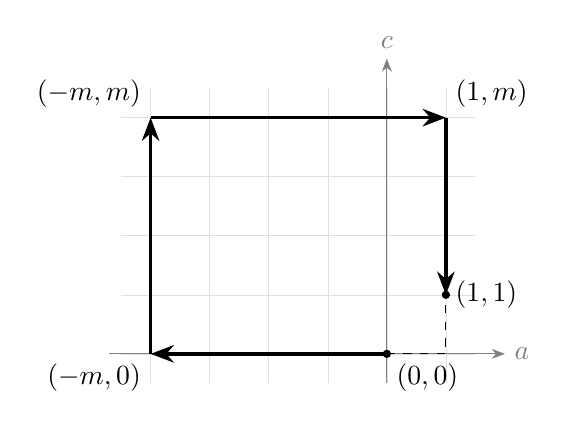
\begin{tikzpicture}[scale=0.75,>=Stealth]
\draw[step=1,gray!25,very thin] (-4.5,-0.5) grid (1.5,4.5);
\draw[->,gray] (-4.7,0)--(2,0) node[right]{$a$};
\draw[->,gray] (0,-0.5)--(0,5) node[above]{$c$};
\draw[very thick,->] (0,0)--(-4,0);
\draw[very thick,->] (-4,0)--(-4,4);
\draw[very thick,->] (-4,4)--(1,4);
\draw[very thick,->] (1,4)--(1,1);
\fill (0,0) circle (2pt) node[below right]{$(0,0)$};
\fill (1,1) circle (2pt) node[right]{$(1,1)$};
\node[below left] at (-4,0){$(-m,0)$};
\node[above left] at (-4,4){$(-m,m)$};
\node[above right] at (1,4){$(1,m)$};
\draw[dashed] (0,0)--(1,0)--(1,1);
\end{tikzpicture}
\caption{The commuting detour $X_m$ (shown at $m=4$). The dashed two-letter
path is $ac$. Every long subpath avoids an identity or single-letter
shortcut, although the whole detour equals this two-letter path.}
\end{figure}

\begin{lemma}[The middle-generator obstruction]\label{lem:doublecoset}
For $p,q\in P=\langle a,c\rangle$, the braid $p b q$ cannot be the identity
or $a^{\pm1}$ or $c^{\pm1}$. It equals a signed middle generator only in
the case
\[
 p b q=b,\qquad p=q=1.
\]
In particular it never equals $b^{-1}$.
\end{lemma}
\begin{proof}
At permutation level let
$H=\langle(12),(34)\rangle$ and $t=(23)$. The double coset $HtH$ is
disjoint from $H$, proving the first assertion. If $p b q=b^{\pm1}$,
then the permutations of $p$ and $q$ lie in
$H\cap tHt^{-1}=\{1\}$. Thus write
$p=a^{2r}c^{2s}$ and $q=a^{2u}c^{2v}$.

Track signed crossings between the original labeled strands. This vector
is invariant under braid relations: cancelling opposite crossings gives
zero; a commuting relation preserves its two labeled pairs; and the braid
relation crosses the same three labeled pairs once on either side.
For a pure power $a^{2r}$ only pair $12$ has count $2r$, and analogously
$c^{2s}$ contributes to pair $34$. Since the permutation of $p$ is the
identity, the middle letter $b$ contributes $+1$ to pair $23$.
After that letter, the contributions from $q$ are $2u$ on pair $13$ and
$2v$ on pair $24$. Equality to $b^{\pm1}$ therefore forces
$r=s=u=v=0$ by the four other pair counts, and the count on pair $23$
forces the positive sign.
\end{proof}

\begin{proof}[Proof of Theorem~\ref{thm:separation}]
A cyclic source interval not containing the unique letter $b$ lies in the
path $X_m$. Lemma~\ref{lem:path} excludes identity and long single-letter
replacements there; a word in $P$ cannot equal $b^{\pm1}$ by permutation.
An interval containing $b$ has the form $p b q$, where $p$ is a suffix of
$X_m$ and $q$ is a prefix. Lemma~\ref{lem:doublecoset} permits a signed-letter
target only when $p=q=1$. Simplicity of the prefix path says that no
nonempty prefix of $X_m$ is the identity and no nonempty suffix has identity
product. Thus the only such interval is the original single letter $b$,
which does not strictly shorten. This proves the radius-one assertion at
all cuts.

Radius two may replace $X_m$ by $ac$, leaving $acb$ of length three.
Its permutation is a four-cycle, so Lemma~\ref{lem:lower} forbids an output
shorter than three. Finally the closure of $acb$ is the unknot: rotate to
$cba$, remove the singleton left endpoint generator $a$ by Markov
destabilization, obtaining a three-braid $\sigma_2\sigma_1$; rotate and
destabilize again, and then remove the remaining two-strand crossing.
Every step preserves the oriented closure type.
\end{proof}

\begin{remark}[What this separation does not prove]
The family has a three-letter \emph{equal braid representative}. A whole-word
Garside normal form immediately exposes a short simple braid. Accordingly
our candidate portfolio handles it before the larger dictionary is built.
The theorem separates the radius-one and radius-two \emph{interval rules};
it is not a lower bound for all braid algorithms, all Garside reductions,
or all unknot recognizers. This distinction is also visible in the timing
table in Section~\ref{sec:experiments}.
\end{remark}

\section{Further obstructions and the role of cyclic closure}

\subsection{Removing the repository's rank-two blind spot}
The maintained rank-two analysis supplies the family
\cite{ProveItRankTwo}
\[
 U=abcaba,\qquad V=cbacbc,\qquad Q_h=(UV^{-1})^h abc\in\B_4.
\]
Both $U$ and $V$ are positive words for $\Delta_4$. Hence $Q_h=abc$,
its closure is the unknot, and its length is $12h+3$.

\begin{proposition}[Unrestricted support removes that obstruction]
For every $h\ge1$,
\[
 \kl{1}(Q_h)=\kc{1}(Q_h)=3.
\]
The original rank-two strictly shortening rule set cannot begin on $Q_h$,
even if it permits longer target words.
\end{proposition}
\begin{proof}
Our rule set deletes the whole identity prefix $(UV^{-1})^h$. The output
$abc$ has a four-cycle permutation, forcing the lower bound three.
For the rank-two obstruction, any subword lying inside a uniform-sign
block is already geodesic by exponent sum. A subword using at most two
indices and crossing a sign boundary is confined to $ac^{-1}$ or
$c^{-1}a$, because the neighboring letters have index $b$. These two-letter
words have two independent commuting exponents and cannot shorten.
\end{proof}

This is an exact extension of the repository's compression capability.
It is not an end-to-end performance claim: the maintained analysis reports
that an earlier descending-diagram certificate already settles its barrier
fixture, and whole-word normalization also exposes the short braid. A new
preprocessing stage should not displace a cheaper certificate merely to
show a favorable isolated benchmark.

\subsection{Geodesic braid representatives of the unknot}
There is a more fundamental obstruction to any method that insists on
preserving the original braid element while seeking a short word.

\begin{theorem}[A geodesic unknot family]\label{thm:geodesic}
In $\B_3=\langle a,b\mid aba=bab\rangle$, let
\[
 G_m=a^{m+1}ba^{-m}\qquad(m\ge1).
\]
Its closure is the unknot, but its minimum Artin word length as the same
braid element is exactly $2m+2$. Consequently no strictly shortening
braid-equality substitution, with any support or any target length, can
start on any subword of $G_m$. Nevertheless,
\[
 \kl{1}(G_m)=2m+2,\qquad \kc{1}(G_m)=2.
\]
\end{theorem}
\begin{proof}
Put $x=aba$, $y=ab$. The presentation becomes
$\langle x,y\mid x^2=y^3\rangle$. Quotienting by the common central
power gives the free product $C_2*C_3$. In this quotient,
\[
 a=y^2x,\quad a^{-1}=xy,\quad b=xy^2,\quad b^{-1}=yx.
\]
The reduced free-product word for $G_m$ is
\[
 (y^2x)^m\,y\,(xy)^m,
\]
which has $4m+1$ syllables. The image of each signed Artin letter has two
syllables before reduction, so every word equal to $G_m$ has length at
least $\lceil(4m+1)/2\rceil=2m+1$. Exponent sum is two; word length must
therefore be even. The lower bound improves to $2m+2$, attained by the
given word. A shortening of a subword would shorten the whole equal braid,
contradicting this geodesicity.

On the other hand, $G_m=a^m(ab)a^{-m}$ is conjugate to $ab$, whose closure
is the unknot by two destabilizations. Rotating after the first $m$ letters
exposes $ab a^{-m}a^m$, and the final identity block may be removed.
Its three-cycle permutation forbids an output shorter than two.
\end{proof}

\begin{corollary}[A limitation on equality-only small-core programs]
No preprocessor whose output must be equal to the original braid element
can guarantee an $O(\log^C n)$-letter output on every unknot braid, for any
fixed $C$. This remains false at the fixed strand count three.
\end{corollary}
\begin{proof}
Apply the geodesic lower bound to $n=2m+2$.
\end{proof}

This does not exclude efficient algorithms operating on compressed objects,
and it does not exclude conjugacy or Markov transformations. In fact the
repository already performs free cyclic cancellation
\cite{ProveItDescent}, so it can remove this particular conjugating sleeve
without the new global optimizer. The theorem isolates a logical
requirement, not an unclaimed new speedup on that input.

\subsection{Hidden sleeves beyond literal free cancellation}
For another test family, let
\[
 u_m=(aba)a^m,\quad v_m=(bab)a^m,\quad
 Z_m=u_m(ab)v_m^{-1}.
\]
Since $u_m=v_m$, a cyclic cut followed by the identity replacement
$v_m^{-1}u_m\mapsto\eps$ proves $\kc{1}(Z_m)=2$.
For $m\ge2$ the written word is freely and cyclically reduced: no adjacent
inverse pair occurs even at the circular seam. Thus free cancellation
alone does not expose every sleeve that the global prefix method finds.

For $2\le m\le16$, the supplied tests additionally find
$\kl{1}(Z_m)=|Z_m|$. This last statement is reported only as a finite
observation, not as a theorem for all $m$. The family lies in three strands,
so a complete closed-three-braid gateway may already decide its closure;
again no complete-recognizer gain is inferred from the kernel output.

Even a four-letter three-braid can be a cyclic radius-one fixed point:
$ba^{-1}ba$ is conjugate to $ab$ by $a^{-1}b^{-1}$, and the tests verify
$\kc{1}=4$, $\kc{2}=2$. The infinite four-strand separation in
Theorem~\ref{thm:separation} supplies the stronger, unbounded version with
a uniform proof.

\section{A constructive quasi-polynomial recognition class}

\subsection{The exact fallback cost}
\begin{lemma}[Conventional exact fallback]\label{lem:fallback}
A $k$-crossing braid diagram with a knot closure admits an exact unknot
recognition algorithm using $\operatorname{poly}(k)2^{O(k)}$ bit operations.
\end{lemma}
\begin{proof}
One route is to construct the reduced rational Khovanov complex and compute
its total homology rank. Its cube has $2^k$ resolutions. For a $b$-strand
braid the number of circles in a resolution is at most $b+k$, and for a
knot closure $b\le k+1$. Thus the total number $N$ of enhanced-state basis
vectors is $2^{O(k)}$. The differential matrices have entries $0,1,-1$.

Exact rational ranks can be computed by fraction-free elimination or an
exact minor-based elimination scheme using a polynomial number of
operations in $N$. Hadamard's determinant bound gives
$O(N\log(N+2))$ bits for the relevant integer minors of these matrices.
Therefore the full bit complexity is still $N^{O(1)}=2^{O(k)}$, with only
polynomial factors in $k$. The chain property gives homology dimensions
from the matrix ranks. Reduced rational Khovanov homology has rank one
exactly for the unknot by Kronheimer--Mrowka \cite{KM2011}.
\end{proof}

This lemma supplies a concrete theoretical fallback, not an unexplained
exponential oracle. The maintained repository uses its own exact homology
pipeline. The distributed new code is a preprocessor and verifier; it does
not reimplement that entire backend or claim that an external smoke test
has been run.

\begin{theorem}[Small-kernel recognition]\label{thm:recognition}
Fix a radius $\rho$. For a braid input whose closure is a knot, run the
uncapped certified radius-$\rho$ kernel or the portfolio of
Proposition~\ref{prop:portfolio}, then use an uncapped exact fallback as in
Lemma~\ref{lem:fallback}. If its output has $k$ letters, the total time is
\[
 \operatorname{poly}_{\rho}(n,b)+\operatorname{poly}(k)2^{O(k)}.
\]
In particular, the algorithm is quasi-polynomial on every family satisfying
\[
 \kc{\rho}(w)=O(\log^2(n+2)):
 \qquad T(n)=2^{O(\log^2(n+2))}=n^{O(\log n)}
\]
for nontrivial growing input sizes.
\end{theorem}
\begin{proof}
Theorems~\ref{thm:optimal}, \ref{thm:cost}, and \ref{thm:replay}
provide the polynomial preprocessing and preservation of closure type.
For the portfolio, its output is no longer than the kernel optimum.
The output permutation remains a single $b$-cycle, so $b\le k+1$.
Diagram construction adds polynomial cost, and Lemma~\ref{lem:fallback}
gives the remaining term. Substitution of the stated bound on $k$ proves
the quasi-polynomial conclusion.
\end{proof}

\subsection{A class whose decomposition is not supplied}
\begin{definition}[Conjugated flat radius-$\rho$ inflation]
Take a core braid word $c$ of length $k_0$ on the same strands and partition
it into consecutive blocks of length at most $\rho$. Replace each block
by a no-shorter word equal to it in the braid group; insert any number of
disjoint identity blocks. Call the result $y$. Finally form
\[
 w=u y v,\qquad vu=1\ \text{in }\B_b.
\]
Neither the partition, the equalities, nor the two sleeve words need be
provided to the optimizer.
\end{definition}

\begin{corollary}[Constructive inflation theorem]\label{cor:inflation}
Every such word satisfies $\kc{\rho}(w)\le k_0$. Hence, when its closure
is a knot and $k_0=O(\log^2(n+2))$, it is recognized in quasi-polynomial
time by the uncapped composition, without a supplied inflation decomposition.
\end{corollary}
\begin{proof}
Rotate to $yvu$. Delete the identity sleeve $vu$, replace the inflated
blocks by their core targets, and remove the inserted identity blocks.
These are disjoint permitted intervals. Blocks that were not lengthened
can simply be retained, so only strictly shortening substitutions are
needed. The plan leaves $c$. Exact optimization finds an output at least
as short as this existing plan without needing to be given it.
\end{proof}

Radius one permits arbitrarily high-support inflation words for individual
letters, extending the previous rank-two setting. Radius two also permits
commuting detours $X_m\mapsto ac$ inside a core, including the strict
separation family. Conjugated versions and disjoint combinations are
covered automatically. No claim is made that every unknot diagram admits
one of these decompositions with a small core.

\subsection{Where the remaining global gap is located}
The theorem is not just a promise that an already supplied short certificate
will be checked: the decomposition is searched for in polynomial time.
Nevertheless, the family hypothesis bounds the output of an explicit
restricted optimization problem. It is not a theorem that the output is
small for arbitrary knot inputs. The geodesic family excludes a universal
equality-only word-length argument; the rectangle family excludes a
universal radius-one interval argument even with all cyclic cuts.

Additional closure-preserving operations, such as independently certified
Markov moves or exchange moves, could enlarge the class. Their search
cost, the number of required moves, and every intermediate representation
size must all be controlled. Merely naming such transformations does not
close the quasi-polynomial proof.

\section{Implementation validation and measurements}\label{sec:experiments}

\subsection{Reproducible finite checks}
The delivered test run contains \textbf{47 passing tests} on CPython 3.13.5.
The retained log records 11.952 seconds for that run; wall times will vary.
Within these tests are the following independent or exhaustive checks.

The normal-form engine is compared with the faithful Artin action on all
5,461 three-braid words through length six and all 1,555 four-braid words
through length four: 7,016 words in total, with collision consistency checked
in both directions. All 872 permutations on two through six strands are
checked as simple braids. Additional seeded tests check 500 independently
expanded normal forms, 300 inverse products, defining relations in 600
contexts, and 100 transfer-potential bounds.

The radius-one optimizer is compared against an exhaustive interval oracle
in 1,162 linear/cyclic instances. The radius-two optimizer adds 350 such
comparisons, for \textbf{1,512 independent optimum comparisons}. These
include repeated or empty inputs where the test definitions generate them;
the count is a number of comparisons, not a count of distinct knots.
The generic radius-one trie implementation is also compared with the
specialized implementation in 300 instances.

Other tests cover rotation equivariance, exact lower-bound stopping,
conjugated inflations, the explicit infinite-family formulas at bounded
parameters, portfolio dominance in 240 radius-specific comparisons, source
association, invalid indices and booleans, overlapping intervals, altered
targets, corrupted proof lengths, and exhausted local allowances.
The tests do not establish an asymptotic theorem by extrapolation; those
bounds rest on the preceding proofs.

\subsection{A paired test of shared versus duplicated algebra}
The primary benchmark compares the shared doubled-prefix engine with a
reference that prepares fresh prefix algebra for every cyclic cut. Both
use the same normal-form implementation, target dictionary, and scalar
dynamic program. The reference generates and replays only the winning
certificate, rather than wasting proof generation at every rotation.
Safe lower-bound stopping is disabled in \emph{both} arms to isolate the
all-cut construction. Imports and input generation are excluded; winning
certificate generation and independent replay are included.

There are seven shuffled paired rounds per case, with two identical shared
arms A and B as an A/A control. Inputs, seeds, per-run times, counters,
verdict-free outputs, and environment details are retained in
\code{data/benchmarks.json}. The host reports Linux x86-64 and an AMD EPYC
9V74 processor. No arm was truncated by a timeout.

\begin{table}[ht]\centering\small
\begin{tabular}{lrrrrrr}
\toprule
Input & $n$ & $k$ & Shared (ms) & Naive (ms) & Ratio & A/A \\
\midrule
single\_crossing & 1 & 1 & 0.02 & 0.02 & 0.87 & 1.03 \\
positive\_4\_braid & 9 & 9 & 0.62 & 2.64 & 4.30 & 1.05 \\
ranktwo\_barrier\_h1 & 15 & 3 & 1.50 & 10.66 & 7.56 & 0.95 \\
ranktwo\_barrier\_h4 & 51 & 3 & 5.89 & 121.08 & 20.56 & 1.02 \\
geodesic\_m12 & 26 & 2 & 10.35 & 61.90 & 5.93 & 1.01 \\
hidden\_sleeve\_m8 & 24 & 2 & 7.83 & 50.68 & 6.33 & 0.95 \\
seeded\_5\_braid & 22 & 6 & 9.61 & 89.04 & 9.27 & 1.01 \\
\bottomrule
\end{tabular}

\caption{Compressor-level all-cut measurements. Times are median milliseconds;
Ratio is the median paired naive/shared-A ratio; A/A is the median paired
shared-B/shared-A ratio. These are not complete-recognizer timings.}
\end{table}

The six multi-crossing fixtures show median paired ratios from about
$4.3$ to $20.6$; the one-crossing fixture shows overhead, with a ratio below
one. The A/A controls are near one but do not constitute a statistical
confidence interval. Exact append counts match
Theorem~\ref{thm:sharedcount}; elapsed ratios differ because height and scalar
work also matter. The input corpus is deliberately small and structured,
not a representative distribution of hard knots.

A separate seven-round run uses the default lower-bound stopping on the
repository's $Q_h$ family. It evaluates only the first cut and attains the
minimum length three. Canonical doubled-prefix height remains two on the
recorded cases.

\begin{table}[ht]\centering\small
\begin{tabular}{rrrrrr}
\toprule
$h$ & $n$ & $k$ & $R$ & Time (ms) & Certificate bytes \\
\midrule
8 & 99 & 3 & 2 & 8.65 & 3324 \\
32 & 387 & 3 & 2 & 34.83 & 12589 \\
128 & 1539 & 3 & 2 & 136.72 & 49646 \\
\bottomrule
\end{tabular}

\caption{Certified radius-one kernel on $Q_h$, with the exact lower-bound
shortcut enabled. Certificate sizes are compact JSON bytes. The separate
whole-word candidate is not included in these kernel timings.}
\end{table}

\subsection{Radius enlargement has a real cost}
The next experiment checks the theorem $\kc{1}(W_m)=4m+1$ versus
$\kc{2}(W_m)=3$ on the rectangular family. It also measures the practical
portfolio, whose whole-word normal-form candidate already attains three.
The two radius arms were shuffled in seven paired rounds. Portfolio times
come from a separate seven-round run and are descriptive medians, not a
paired speedup estimate. All three measurements include their required
independent replay.

\begin{table}[ht]\centering\small
\begin{tabular}{rrrrrrr}
\toprule
$m$ & $n$ & $\kappa_1$ & $\kappa_2$ & Radius 1 & Radius 2 & Portfolio \\
\midrule
2 & 9 & 9 & 3 & 1.24 & 7.69 & 0.22 \\
8 & 33 & 33 & 3 & 15.67 & 94.82 & 1.91 \\
32 & 129 & 129 & 3 & 229.99 & 1369.98 & 28.78 \\
\bottomrule
\end{tabular}

\caption{Rectangular-family outputs and median times in milliseconds.
The two kernel arms solve different optimization problems. The portfolio
returns a three-letter equal braid without constructing the larger target
query table.}
\end{table}

Radius two pays substantial dictionary and normal-form overhead even though
it finds a dramatically shorter kernel. On the $129$-letter example its
median is about $1.37$ seconds, versus about $0.23$ seconds for an unchanged
radius-one kernel. The cheap portfolio instead takes about $29$ milliseconds.
No elapsed full-recognizer gain follows from those numbers: an upstream
structural certificate might already recognize the knot faster. Conversely,
comparing unchanged and shortened kernel times alone ignores the possible
cost of a later exact homology computation. Both facts are why end-to-end
measurements are required before changing defaults.

\subsection{What has not been executed}
The complete ProveIt test suite was not run in this environment. The
repository was inspected through the GitHub connector at the recorded
snapshot, but a full local checkout was not available. Thus the upstream
suite's reported 272 passing tests are source-reported status, not a claim
of a new run here \cite{ProveItReadme}. The optional supplied upstream smoke
script is marked unexecuted. No Rust integration or Lean formalization is
claimed, and no public repository files were modified.

\section{Integration into the maintained recognizer}

\subsection{Placement and provenance}
The proposed package is additive and optional. Keep existing inexpensive
certificates, free cyclic cleanup, singleton endpoint destabilization, and
the specialized rank-two stage ahead of a potentially expensive global
probe. Exact whole-word normalization is the first stage of the proposed
portfolio; an unrestricted cyclic kernel follows only if needed.

The current \code{Diagram.braid_source} property identifies a checked source
braid; it is not an unchecked auxiliary input. A probe must operate on that
source, independently replay its candidate, and construct a replacement
\code{Diagram.from_braid} only when it improves on the \emph{current}
simplified diagram's crossing count. Otherwise it should retain the existing
pipeline state. Earlier planar-diagram reductions and a restarted source
braid belong to different evidence branches. A cyclic braid certificate
connects them through the original source, not by pretending to be a
concatenated Reidemeister move trace.

The supplied optional adapter follows this pattern. It is not wired into
the maintained recognition function. It supplies a candidate and evidence,
not a knot verdict. An adopter must preserve the recognizer's remaining global
budget, avoid recursively re-enabling the same probe on restart, and retain
all existing fallback and provenance rules.

\subsection{Failure behavior}
A local search limit or dictionary cap is inconclusive: discard the probe
and continue from the unchanged input. Global budget exhaustion remains
\code{UNKNOWN} under the host recognizer's contract. An invalid replay is
an implementation error to investigate, never evidence for knot or unknot.
The conditional complexity theorem applies when the relevant local and
fallback caps are removed; bounded production runs can return inconclusive
results and are not silently substituted for the theorem's algorithm.

The candidate portfolio uses only a single certificate rooted at the
original word. If future versions repeatedly alternate diagram reduction,
normalization, and cyclic kernels, a provenance graph or explicit sequence
of source-to-source certificates will be necessary. Those additional passes
must be counted separately.

\section{Further research questions}

\paragraph{1. A strict hierarchy beyond radius two.}
For each fixed $\rho$, construct and prove an infinite unknot family with
$\kc{\rho}(w)=\Omega(|w|)$ but $\kc{\rho+1}(w)=O(1)$, or determine where
such a statement fails. The lattice construction proves the first step.
A stronger and more practically relevant version should remain difficult
after whole-word normal-form expansion and cheap Markov descent. Our
rectangle family does not meet that stronger condition.

\paragraph{2. Reuse scalar work between adjacent cuts.}
Theorem~\ref{thm:sharedcount} removes repeated braid algebra, not the
$O(n^2M)$ scalar term. Can the interval-state structure support a rolling
maximum, persistent dynamic program, or a specialized min-plus algorithm
that reuses more work between cuts? Any proposed update must handle the
changed left boundary and the loss of old maximizing starts exactly.

\paragraph{3. Persistent canonical states with a lazy half-twist action.}
The prototype copies simple-factor lists and applies $\tau$ eagerly on
negative input. Persistent trees, lazy involutions, and local left-weighting
may reduce this overhead. A useful next theorem would bound update work in
terms of the actual changed normal-form suffix, with a deterministic
comparison and memory model rather than unverified hash equivalence.

\paragraph{4. Implicit targets for commuting powers and parabolic blocks.}
A literal radius ball is expensive. Can families such as $a^pc^q$,
short geodesics in a small parabolic subgroup, or simple braids be queried
without enumerating all target words? The output cost must remain actual
Artin length or another explicitly justified objective. The empty-target
and one-letter table is insufficient for the rectangular detours.

\paragraph{5. Closure-aware operations with controlled search.}
Combine the portfolio with certified destabilization, exchange moves,
conjugation changes not visible as literal cuts, and selected
length-preserving relations. Identify families on which the number of
rounds and all intermediate sizes are bounded. The geodesic theorem
explains why equality-only kernels cannot be the whole strategy.

\paragraph{6. A structural bridge to the quasi-polynomial target.}
Prove that a meaningful, naturally described class of unknot diagrams
admits a polynomially constructible sequence leading either to a
$O(\log^2 n)$ kernel or to a compressed exact-homology calculation with a
quasi-polynomial size bound. No universal bound on braid index, scan
multiplicity, or kernel size should be inserted without proof.

\paragraph{7. Proof compression and formal verification.}
Formalize the simple-transfer invariant and residual replay theorem,
then the last-interval optimality induction. Compress repeated transfer
segments using a checked straight-line proof language. Such compression
must preserve a polynomial verifier and must not move an unbounded
normal-form computation into the trusted checker unnoticed.

\paragraph{8. Complete-recognizer evaluation.}
Run the optional stage against a pinned checkout, preserving cheap
certificates and time accounting. Use shuffled paired end-to-end runs,
A/A controls, memory measurements with censoring reported, and a corpus
including cases where each probe fails. Report output-size improvement
separately from actual time-to-verdict. The included local data are a
starting point, not a substitute for this evaluation.

\section{Conclusion}
The new layer gives exact support-unrestricted braid compression, shared
cyclic-prefix arithmetic, finite-target trie sharing, and independently
replayable transformations with explicit complexity bounds. The infinite
rectangle family proves that target radius matters even after all supports
and all literal cyclic cuts have been allowed. The geodesic family proves
that original-braid equality alone cannot universally produce short unknot
words. Both negative results sharpen the design requirements instead of
being hidden by successful examples.

The constructive positive result is an uncapped quasi-polynomial
recognizer for the stated small-kernel and conjugated-inflation classes.
The practical result is an opt-in, tested preprocessor with a cheap
normal-form shortcut and measured shared-algebra savings. The general
quasi-polynomial problem still requires an additional structural theorem
or a different compressed representation with a complete cost proof.

\appendix
\section{Reproduction and artifact map}
The package is standard-library Python 3.10+ and was tested under 3.13.5.
No network access or third-party Python package is needed for its tests.
From the unpacked package root:
\begin{lstlisting}
python -m unittest discover -s tests -v
python scripts/benchmark.py --rounds 7
python scripts/radius_experiment.py
python -m cyclic_garside compress certificates/rectangle_m2.json \
    --radius 2 -o result.json
python -m cyclic_garside verify certificates/rectangle_m2.json result.json
cd docs && sh build.sh
\end{lstlisting}
The Python API separates a rule-set optimum from a practical portfolio:
\begin{lstlisting}[language=Python]
from cyclic_garside import compress, compress_radius, preprocess
from cyclic_garside import verify, verify_radius

# Optimal support-unrestricted radius-one cyclic interval plan.
result = compress(4, word)
verify(4, word, result["certificate"])

# Optimal radius-two plan; dictionary allocation is explicitly capped.
result = compress_radius(4, word, radius=2, max_targets=100000)
verify_radius(4, word, result["certificate"])

# Cheap whole-word candidate first, then a cyclic kernel if necessary.
# This output is not labeled as a radius-specific optimum.
result = preprocess(4, word, radius=2)
\end{lstlisting}

The artifact directories contain source code, independent oracles and tests,
raw benchmark JSON, example certificates, this article and build sources,
an exact source manifest, an integration adapter and an unexecuted upstream
smoke script. The JSON schema is intentionally small and versioned; the
verifier is the authoritative executable check of its local moves.
The SHA-256 manifest covers the released artifact bytes, not a cryptographic
endorsement of their mathematical claims.

\section{Audit questions for a reviewer}
A review can proceed without trusting the timing conclusions. First check
the two permutation conventions in Lemma~\ref{lem:transfer}; reversing
starting and finishing sets is a plausible implementation error. Next check
the negative-letter complement and the movement of $\Delta^{-1}$ to the
left. Then verify that both certificate implementations reconstruct their
actual source and never accept permutation equality as braid equality.

For the optimizer, the critical identities are
$P_i=P_jv^{-1}$ and the query-before-insertion recurrence. For the cost
proof, inspect negative updates, list deletions, target trie size, proof
allocation, and the distinction between word and bit operations. For the
separation theorem, verify the induced path and the labeled-pair crossing
calculation across the unique $b$. For the recognition theorem, check that
strand count is removed using the one-cycle permutation and that the
fallback uses an actual exact homology calculation rather than an assumed
short certificate.

Independent finite checks have deliberately been included for these seams.
No test outcome should be used to replace a missing all-input proof, and no
source-reported upstream test count should be mistaken for an executed
integration test.

\begin{thebibliography}{9}
\bibitem{Dehornoy2007}
P. Dehornoy, \emph{Efficient solutions to the braid isotopy problem},
arXiv:math/0703666 (2007), especially the simple-braid model and greedy
normal form in Section 1.
\url{https://arxiv.org/abs/math/0703666}.

\bibitem{KM2011}
P. B. Kronheimer and T. S. Mrowka,
\emph{Khovanov homology is an unknot-detector},
Publications Math\'ematiques de l'IH\'ES \textbf{113} (2011), 97--208;
arXiv:1005.4346.
\url{https://arxiv.org/abs/1005.4346}.

\bibitem{Lackenby2026}
M. Lackenby, \emph{Incompressible surfaces, hierarchies and unknot recognition},
arXiv:2607.23350v1 (2026), Section 9.
\url{https://arxiv.org/abs/2607.23350}.

\bibitem{ProveItReadme}
V. Reshetnikov, \emph{ProveIt: Topology/UnknotRecognition, README},
inspected blob \code{46709747407df3853298bf42ec1566c6ef836f3a},
October 2026. Exact source paths and snapshot metadata are supplied in
\code{source_manifest.json}.
\url{https://github.com/VladimirReshetnikov/ProveIt/tree/main/Topology/UnknotRecognition}.

\bibitem{ProveItRankTwo}
ProveIt research program, \emph{Verified rank-two braid preprocessing},
\code{synthesis/ranktwo.tex}, inspected blob
\code{bd2943b64959697790fc71974a5442250710641d}.
\url{https://github.com/VladimirReshetnikov/ProveIt/blob/main/Topology/UnknotRecognition/synthesis/ranktwo.tex}.

\bibitem{ProveItDescent}
ProveIt research program, \emph{Checked elementary Markov descent},
\code{fast/fastunknot/braid_reduction.py}, inspected at commit
\code{a70135c01af3d106cec88045fa6ba8dd7d2ee0f1}.
\url{https://github.com/VladimirReshetnikov/ProveIt/blob/main/Topology/UnknotRecognition/fast/fastunknot/braid_reduction.py}.

\bibitem{OpenAIRestriction}
OpenAI, \emph{Positive braid derivations restrict to a full subdiagram},
\code{lean/OAI/Topology/ArtinGroups/ParabolicIntersections/BraidRestriction.lean},
commit \code{adc7f1241b42e322a6451854ab7e4b4c146bf78a}.
\url{https://github.com/openai/math}. Inspected as methodological context;
no additional result from this file is assumed in the proofs above.
\end{thebibliography}
\end{document}
